\chapter{Arsitektur Solusi}

Komponen \textit{backend} utama bersifat \textit{stateless}, sehingga dapat di-\textit{scale} dengan meningkatkan jumlah \textit{instance}. Setiap arsitektur solusi memiliki dua layanan eksternal, yaitu layanan pengguna dan layanan gerbang pembayaran. Basis data merupakan komponen yang sulit di-\textit{scale} secara dinamis berdasarkan beban yang diterima. Biasanya, penskalaan secara vertikal merupakan opsi utama untuk meningkatkan \textit{throughput}.

\section{Arsitektur Dasar Acuan}

\begin{figure}[ht]
    \centering
    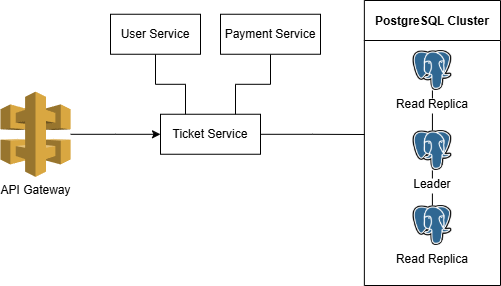
\includegraphics[width=0.8\textwidth]{resources/chapter-3/architecture-reference.png}
    \caption{Arsitektur Dasar Acuan}
    \label{fig:baseline-architecture}
\end{figure}

Arsitektur ini akan menjadi dasar acuan yang digunakan sebagai dasar perbandingan kinerja. Terdapat kluster PostgreSQL dengan konfigurasi satu node pemimpin dan sisanya node replika. Keberadaan replika memungkinkan peningkatan \textit{throughput} permintaan baca, tetapi tidak ada pengoptimalan untuk operasi tulis.

\section{Arsitektur yang Mengoptimalkan PostgreSQL}

Arsitektur ini mengoptimalkan sistem dengan pola CQRS. Tanggung jawab permintaan baca dilimpahkan kepada RisingWave. \textit{Streaming database} ini mengonsumsi \textit{CDC stream} dari kluster PostgreSQL, lalu memperbarui kueri secara inkremental. Penggunaan ekstensi Citus memungkinkan pembagian data berdasarkan baris dan \textit{multiple writer}. Selain itu, perintah pemesanan tiket (berupa \textit{command}/ \textit{event sourcing}) akan dimasukkan ke dalam antrean terlebih dahulu, lalu diproses secara bertahap. Redis digunakan untuk menyimpan \textit{uncommited data} dan menolak permintaan pemesanan lebih awal.

\begin{figure}[ht]
    \centering
    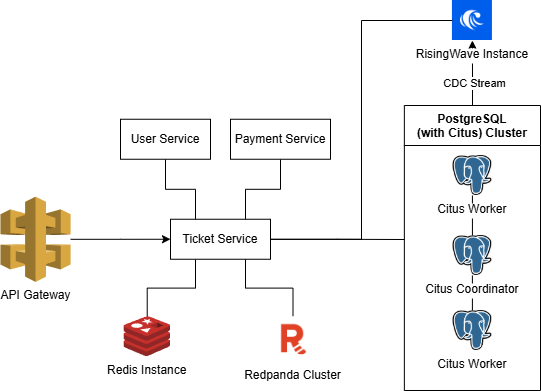
\includegraphics[width=0.8\textwidth]{resources/chapter-3/architecture-optimized.png}
    \caption{Arsitektur yang Mengoptimalkan PostgreSQL}
    \label{fig:optimized-architecture}
\end{figure}

Penggunaan ekstensi Citus memungkinkan penginkatan \textit{write throughput} tidak hanya dengan pendekatan \textit{scale up}, tetapi juga dengan pendekatan \textit{scale-out}. Redpanda dapat dibuat kluster dengan pemartisian data untuk meningkatkan \textit{throughput}. Redis dapat dikonfigurasikan dalam mode kluster untuk redundansi dan mode AOF untuk \textit{persistence}.

\section{Arsitektur \textit{Event-Driven}}

Arsitektur ini tidak menggunakan PostgreSQL sama sekali. Pada dasarnya, basis data relasional terdiri atas komponen \textit{storage} dan \textit{query processor}. Pada arsitektur ini, komponen \textit{storage} diganti menggunakan Redpanda dengan berbagai topik dan \textit{query processor} diganti dengan RisingWave. Meskipun begitu, pendekatan ini tidak memiliki dukungan \textit{transaction} selain \textit{transaction} pada Redpanda yang berupa \textit{push log all or nothing} pada beberapa topik sekaligus. Untuk itu, Redis digunakan untuk menyimpan \textit{dirty data} atau \textit{uncommited data} sehingga untuk mencegah \textit{double booking}.

\begin{figure}[ht]
    \centering
    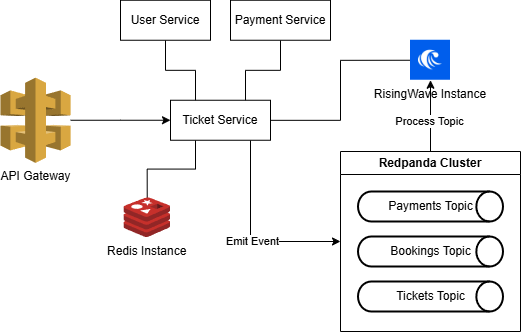
\includegraphics[width=0.8\textwidth]{resources/chapter-3/architecture-event-driven.png}
    \caption{Arsitektur \textit{Event-Driven}}
    \label{fig:solution-event-driven-architecture}
\end{figure}

Redpanda dapat dibuat kluster dengan pemartisian data untuk meningkatkan \textit{throughput}. Redis dapat dikonfigurasikan dalam mode kluster untuk redundansi dan mode AOF untuk \textit{persistence}. Selain itu, RisingWave merupakan \textit{streaming database} yang \textit{cloud-native} sehingga dapat di-\textit{scale out} dengan mudah untuk meningkatkan \textit{throughput}.

